\subsection{Giới thiệu về vector}
Giả sử bạn cần mô tả cho người khác vị trí của một hòn đá. Lấy vị trí của bạn làm gốc, vị trí đó có thể được mô tả bởi một cặp số \((3;4)\), nghĩa là từ chỗ bạn đi \(3m\) về hướng Bắc, rồi \(4m\) về hướng Đông sẽ đến được chỗ hòn đá. Hoặc, bạn có thể chỉ tay vào hòn đá và nói "Hòn đá kia cách tôi \(5m\)" (nếu trước nó có một hòn đá khác cách bạn \(4.5m\), chẳng hạn). 
\begin{figure}[H]
\centering
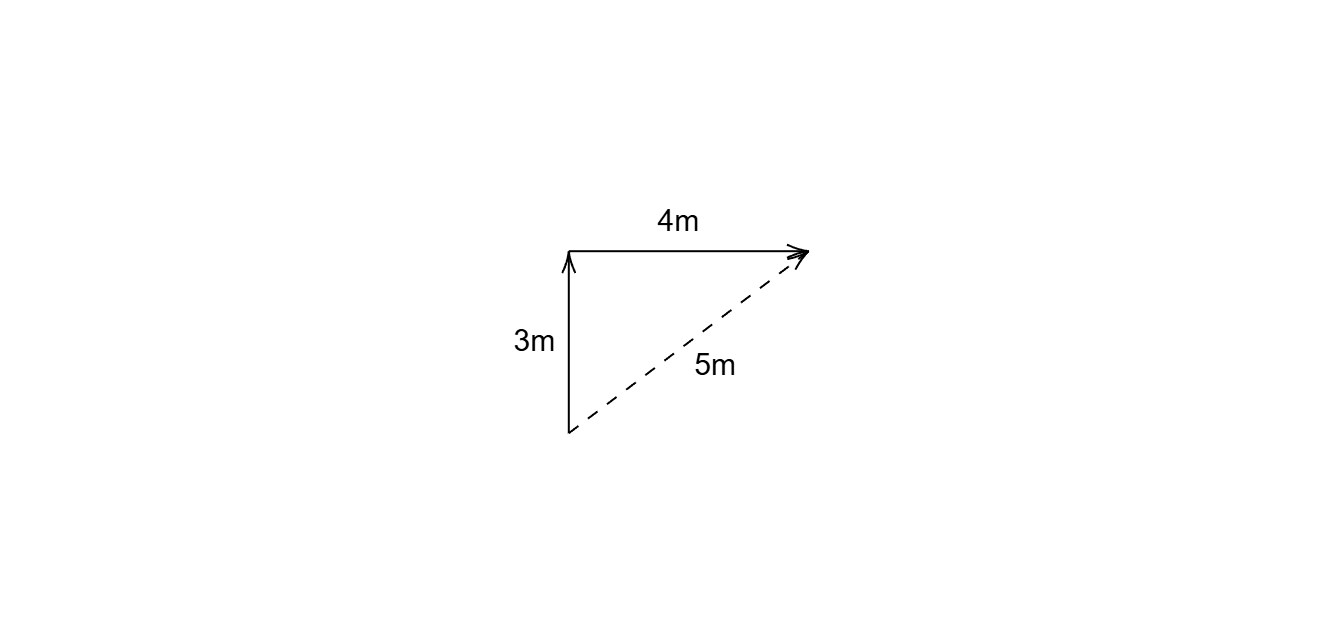
\includegraphics[width=1\textwidth]{Tuan2/Figures/gioithieuvector.png}
\end{figure}
Như vậy nhằm truyền tải những thông tin như vị trí của một vật, ta cần một mảng số (trong trường hợp vừa rồi là một mảng số có hai thành phần), hoặc một cách khác, là \emph{chỉ} về vật thể và xác định rõ ràng khoảng cách. Rõ ràng là kiểu thông tin này không giống với "quãng đường cần đi là 7m", hay "nhiệt độ hôm nay là 30 độ C", được truyền tải thông qua chỉ một con số (và dơn vị). Ta cần một đại lượng có khả năng truyền tải nhiều thông tin hơn để mô tả những 
dạng thông tin phức tạp hơn vậy. Nó được gọi là \textbf{vector}.
\begin{definition} Vector \(AB\) (hình vẽ), kí hiệu là \(\mathbf{AB}\), là một đại lượng biểu diễn bằng mũi tên tuân theo quy tắc hình bình hành được đặc trưng bởi độ dài \(a\) của nó (do đó còn được kí hiệu là \(\vec{a}\)) và hướng mà nó chỉ.
\end{definition}
\begin{figure}[H]
\centering

\includegraphics[width=1\textwidth]{Tuan2/Figures/vectorAB.png}
\end{figure}Đây là một định nghĩa thuần tuý hình học, nhưng sẽ ổn nếu bắt đầu với nó. Một mũi tên chỉ hướng với độ dài xác định là tương đương với một mảng số, như được trình bày trong ví dụ trên. Trong phần này, ta sẽ chủ yếu tập trung vào ý nghĩa hình học của vector , trực quan và không đi sâu vào khía cạnh toán.
Chỉ với định nghĩa này, các đại lượng phức tạp như lực, vận tốc cũng đã có thể được mô tả. Rõ ràng, chúng không thể được xác định chỉ với một con số như khối lượng hay nhiệt độ; vận tốc, lực, hay bất kỳ một đại lượng vector nào khác trong vật lý đều có \emph{hướng} và \emph{độ lớn}. Sau đây ta cũng thống nhất sẽ kí hiệu vector là \(\mathbf{a}\) thay vì \(\vec a\).
\vspace{8pt}

Để so sánh hai vector, ta dựa trên các tiêu chí sau:
    \begin{itemize}
        \item Hai vector \(\mathbf{a}\) và \(\mathbf{b}\) được coi là bằng nhau nếu chúng có cùng độ dài và cùng hướng, kí hiệu là \(\mathbf{a}=\mathbf{b}\).
        \item Hai vector \(\mathbf{a}\) và \(\mathbf{b}\) là đồng phương nếu chúng song song.
        \item Hai vector \(\mathbf{a}\) và \(\mathbf{b}\) có cùng giá nếu chúng cùng nằm trên một đường thẳng, và là đồng phẳng nếu cùng nằm trên một mặt phẳng.
    \end{itemize}

Ngoài ra, để kí hiệu độ lớn của một vector, ta viết \(\lvert \mathbf{a}\rvert\), ngắn gọn là \(a\) nếu không có gì nhầm lẫn.  
\subsection{Các phép toán trên vector}

\subsubsection{Phép cộng vector}
Tưởng tượng để xác định vị trí của viên đá, thay vì xác định trực tiếp, bạn xác định vị trí của Hirrus, và Hirrus xác định vị trí của viên đá. Từ đó, vị trí của nhân vật này được xác định bởi một vector có gốc ở vị trí của ta, đầu ở chỗ của Hirrus; vị trí của viên đá đối với Hirrus lại được xác định bởi một mũi tên có gốc đặt tại chỗ của Hirrus, đầu ở chỗ của viên đá. Đồng thời, vị trí của viên đá đối với bạn được xác định bởi một mũi tên có gốc ở vị trí của bạn, đầu ở chỗ của viên đá. Mũi tên này là kết quả của phép cộng hai mũi tên trước đó, và được gọi là \textbf{phép cộng vector}.
\begin{figure}[H]
    \centering
    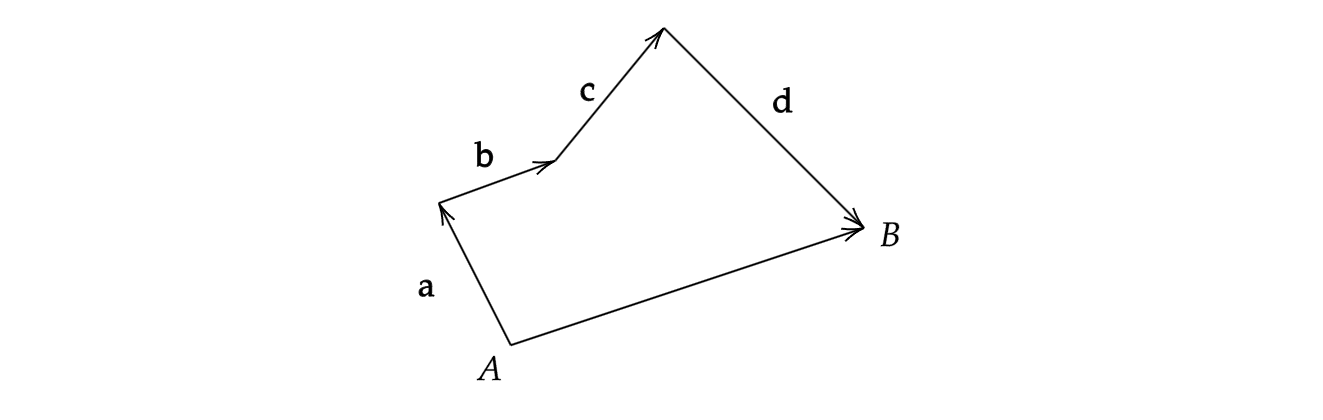
\includegraphics[width=1\textwidth]{Tuan2/Figures/congvector.png}
    \caption{$\mathbf{a}+\mathbf{b}+\mathbf{c}+\mathbf{d}=\mathbf{AB}$}
\end{figure}
Chú ý rằng, về tổng quát, \(\lvert \mathbf{a}+\mathbf{b}\rvert\neq a+b\).
\subsubsection{Tích một vector với một đại lượng vô hướng}
Khi nhân một vector với một đại lượng vô hướng, độ dài của vector sẽ được nhân lên với hệ số bằng đại lượng đó, trong khi hướng của vector không đổi nếu số đó là số dương, đảo chiều nếu số đó là số âm. Đặc biệt, nếu một vector nhân với \(0\), kết quả là vector \(\mathbf{0}=\mathbf{a}+(-\mathbf{a})\).
\begin{figure}[H]
    \centering
    
\includegraphics[width=1\textwidth]{Tuan2/Figures/vector x vo huong.png}
    \caption{phép nhân vector với một đại lượng vô hướng}
\end{figure}

\subsubsection{Tích vô hướng hai vector}
Phép nhân vô hướng hai vector \(\mathbf{a}\) và \(\mathbf{b}\) có kết quả là một đại lượng vô hướng có giá trị bằng:
\begin{equation}
    \mathbf{a} \cdot \mathbf{b} = |\mathbf{a}| |\mathbf{b}| \cos (\mathbf{a}, \mathbf{b})
\end{equation}
Trong đó, \(\cos (\mathbf{a}, \mathbf{b})\) chỉ góc giữa hai vector \(\mathbf{a} \text{ và }\mathbf{b}\).
Ý nghĩa của phép nhân vô hướng được thể hiện như hình vẽ:
\begin{figure}[H]
    \centering
    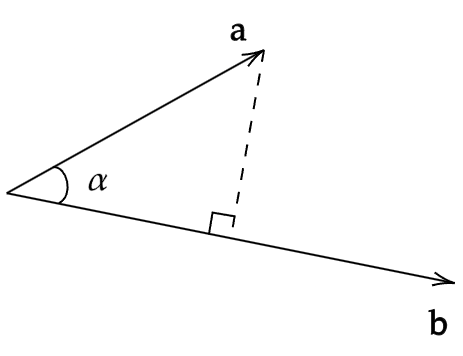
\includegraphics[width=1\textwidth]{Tuan2/Figures/tichcham.png}
    \caption{phép nhân vô hướng hai vector}
\end{figure}
\subsubsection{Tích có hướng hai vector}
Phép nhân có hướng hai vector \(\mathbf{a}\) và \(\mathbf{b}\) có kết quả là một vector hướng vuông góc với mặt phẳng chứa hai vector này:
\begin{figure}[H]
    \centering
    
\includegraphics[width=1\textwidth]{Tuan2/Figures/tichcheo.png}
    \caption{phép nhân có hướng hai vector}
\end{figure}
Vector này có độ dài bằng:
\begin{equation}
    |\mathbf{a} \times \mathbf{b}| = |\mathbf{a}| |\mathbf{b}| \sin (\mathbf{a}, \mathbf{b})
\end{equation}
Chiều của vector này, theo quy ước,  được xác định bằng quy tắc bàn tay phải, hoặc quy tắc vặn nút chai (như hình vẽ).


\subsection{Đạo hàm vector}
\begin{definition}
    Cho \(\mathbf{u}(t)\) là một hàm vector. Đạo hàm của hàm vector này tại điểm \(t_0\) được định nghĩa là:
    \begin{equation}
        \mathbf{u}'(t_0) = \lim_{t \to t_0} \frac{\mathbf{u}(t) - \mathbf{u}(t_0)}{t - t_0}
    \end{equation}
\end{definition}
Cũng giống như đạo hàm của một hàm số, đạo hàm của một hàm vector cũng có một số tính chất đặc biệt:
\begin{itemize}
\item Nếu \(\mathbf{w}(t)=a(t)\mathbf{u}(t)\), thì \(\dfrac{d\mathbf{w}}{dt} = a'(t)\mathbf{u}(t) + a(t)\dfrac{d\mathbf{u}}{dt}\)
\item Nếu \(\mathbf{w}(t)=\mathbf{u}(t) + \mathbf{v}(t)\), thì \(\dfrac{d\mathbf{w}}{dt} = \dfrac{d\mathbf{u}}{dt} + \dfrac{d\mathbf{v}}{dt}\)
\item Nếu \(\mathbf{w}(t)=\mathbf{u}(t) \cdot \mathbf{v}(t)\), thì \(\dfrac{d\mathbf{w}}{dt} = \dfrac{d\mathbf{u}}{dt} \cdot \mathbf{v}(t) + \mathbf{u}(t) \cdot \dfrac{d\mathbf{v}}{dt}\)
\item Nếu \(\mathbf{w}(t)=\mathbf{u}(t) \times \mathbf{v}(t)\), thì \(\dfrac{d\mathbf{w}}{dt} = \dfrac{d\mathbf{u}}{dt} \times \mathbf{v}(t) + \mathbf{u}(t) \times \dfrac{d\mathbf{v}}{dt}\)
\end{itemize}

\subsection{Cơ sở vector}
\subsubsection{Vector đơn vị}
Một vector đơn vị là một vector có độ dài bằng 1. Vector đơn vị thường được sử dụng để biểu diễn hướng của một vector khác. Ví dụ, nếu \(\mathbf{a}\) là một vector bất kỳ, thì vector đơn vị theo hướng của \(\mathbf{a}\) được tính bằng:
\begin{equation}
    \mathbf{u} = \frac{\mathbf{a}}{|\mathbf{a}|} 
\end{equation}
Vector này có độ dài bằng 1 và cùng hướng với \(\mathbf{a}\).
\subsubsection{Cơ sở vector}
Trong không gian ba chiều, một vector cơ sở chuẩn hóa là tập hợp của ba vector đơn vị không đồng phẳng. Một vector có thể được xác định bằng cách biểu diễn nó dưới dạng tổ hợp tuyến tính của các vector đơn vị trong cơ sở.
\begin{equation}
    \mathbf{u}=a\mathbf{e}_1+b\mathbf{e}_2+c\mathbf{e}_3
\end{equation}
\begin{figure}[H]
    \centering
    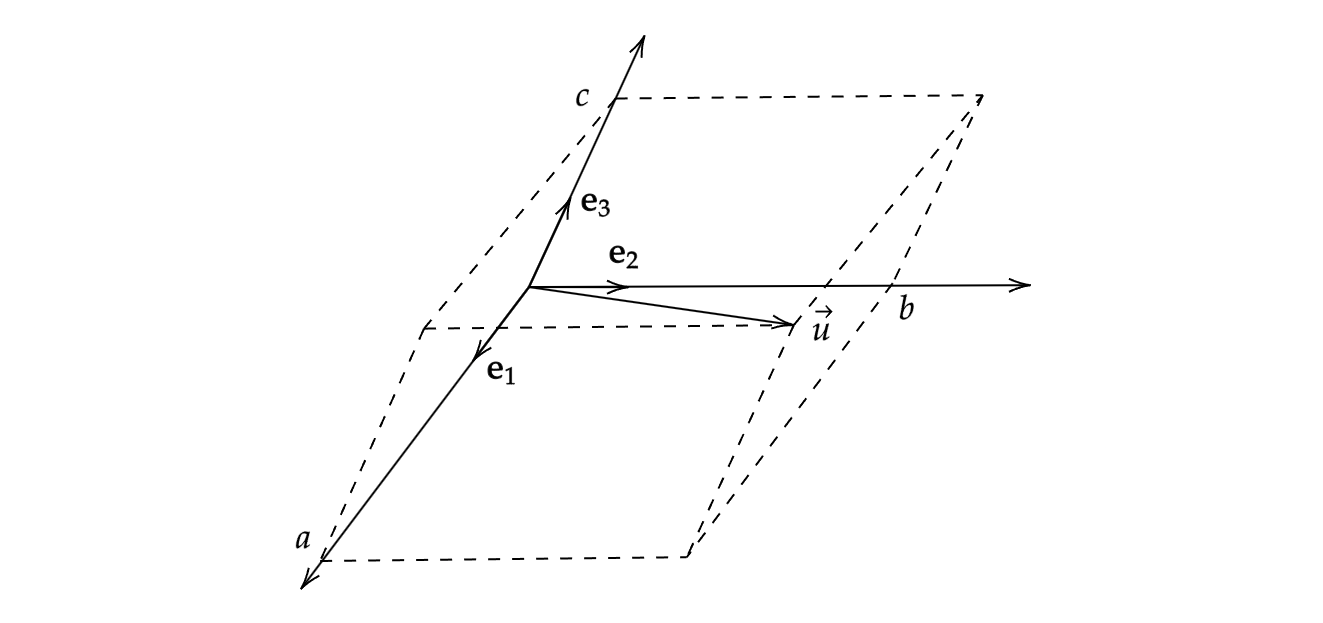
\includegraphics[width=1\textwidth]{Tuan2/Figures/cosovector.png}
    \caption{Cơ sở \((\mathbf{e}_1, \mathbf{e}_2, \mathbf{e}_3)\)}
\end{figure}
Tương tự, trong không gian hai chiều, một vector cơ sở chuẩn hóa là tập hợp của hai vector đơn vị không nằm trên cùng một đường thẳng. Một vector trong mặt phẳng có thể được biểu diễn dưới dạng tổ hợp tuyến tính của các vector đơn vị trong cơ sở:
\[\mathbf{v}=a\mathbf{e}_1 +b\mathbf{e}_2.\]
Xét một vector khác, \(\mathbf{w}=c\mathbf{e}_1 +d\mathbf{e}_2\), vậy \[\mathbf{v}+\mathbf{w}=(a+c)\mathbf{e}_1 +(b+d)\mathbf{e}_2 .\]
Điều này nghĩa là, để đến vị trí được xác định bởi vector \(\mathbf{v}+\mathbf{w}\), ta đi từ vị trí ban đầu theo hướng của \(\mathbf{e}_1\) một khoảng bằng \(a+c\), rồi theo hướng của \(\mathbf{e}_2\) một khoảng bằng \(b+d\). Quay lại ví dụ ban đầu, ta thấy rằng nếu biết sẵn thông tin của \(\mathbf{e}_1\) và \(\mathbf{e}_2\), \(\mathbf{v}+\mathbf{w}\) được xác định qua mảng số \((a+c,b+d)\); 
tương tự, có thể viết \(\mathbf{v}=(a,b)\) hay \(\mathbf{w}=(c,d)\) để \(\mathbf{v}+\mathbf{w}=(a+c,b+d)\). \(a\) và \(b\) được gọi là các \emph{toạ độ} của vector \(\mathbf{v}\), cũng như \(c\) và \(d\) được gọi là các toạ độ của \(\mathbf{w}\).
\vspace{8pt}

Chú ý rằng các vector cơ sở cũng có toạ độ. Cụ thể, \((1,0)\) là toạ độ của \(\mathbf{e}_1\), và (\(0,1\)) là toạ độ của \(\mathbf{e}_2\). Trong trường hợp ba chiều, \(\mathbf{e}_1\), \(\mathbf{e}_2\), và \(\mathbf{e}_3\) có toạ độ lần lượt là \((1,0,0), (0,1,0), (0,0,1)\).

\subsection{Hệ tọa độ Descartes}
\begin{definition}
    Hệ tọa độ Descartes là một hệ tọa độ trực chuẩn, được xác định bởi một gốc tọa độ \(O\) và một vector cơ sở trực chuẩn (\(\mathbf{e}_1, \mathbf{e}_2, \mathbf{e}_3\)). Trong hệ tọa độ này, một điểm \(M\) trong không gian được xác định bởi ba tọa độ \((x, y, z)=(r_1, r_2, r_3)\),
    \begin{equation}
        \mathbf{r}=\mathbf{OM} = x\mathbf{e}_1 + y\mathbf{e}_2 + z\mathbf{e}_3.
    \end{equation}
\end{definition}
\begin{figure}[H]
    \centering
    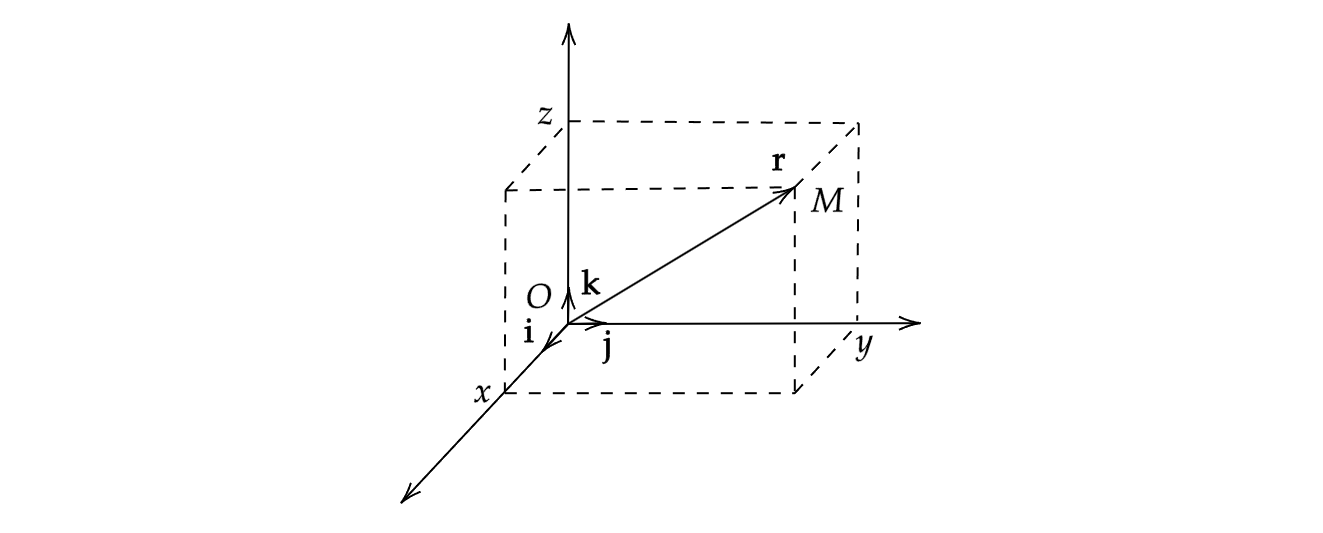
\includegraphics[width=1\textwidth]{Tuan2/Figures/toadodescartes.png}
    \caption{Hệ tọa độ Descartes}
\end{figure}
Trực chuẩn có nghĩa là các vector trong vector cơ sở có độ dài bằng 1 và vuông góc lẫn nhau. Nói cách khác, 
\begin{equation}
    \mathbf{e}_i \cdot \mathbf{e}_j =\delta_{ij}.
\end{equation}
Trong đó, \begin{equation*}
\begin{array}{l}
     \delta_{ij}=\Bigg\{
    \begin{array}{ll}
      1  & \text{, nếu } i=j. \\
      0  & \text{, nếu } i\neq j.
    \end{array}
\end{array}
\end{equation*} được gọi là ký hiệu Kronecker. Như vậy, tích vô hướng của hai vector \(\mathbf{a}=(a_1, a_2, a_3)\) và \(\mathbf{b}=(b_1,b_2,b_3)\) trong hệ tọa độ Descartes có thể được tính bằng công thức:
\begin{equation}
    \mathbf{a}\cdot\mathbf{b}=\sum_{i=1}^{3} a_m b_m = a_1 b_1 + a_2 b_2 + a_3 b_3.
\end{equation} Dễ thấy, \(\mathbf{a} \cdot \mathbf{e}_m =a_m\), nghĩa là thành phần thứ \(m\) của vector \(\mathbf{a}\) chính là tích vô hướng của \(\mathbf{a}\) với vector cơ sở thứ \(m\).
Đồng thời, ta cũng có 
\begin{align*}
\mathbf{e}_1 \times \mathbf{e}_1 = \mathbf{0},    && \mathbf{e}_1 \times \mathbf{e}_2 = \mathbf{e}_3,  && \mathbf{e}_1 \times \mathbf{e}_3 = -\mathbf{e}_2, \\
\mathbf{e}_2 \times \mathbf{e}_1 = -\mathbf{e}_3, && \mathbf{e}_2 \times \mathbf{e}_2 = \mathbf{0},    && \mathbf{e}_2 \times \mathbf{e}_3 = \mathbf{e}_1, \\
\mathbf{e}_3 \times \mathbf{e}_1 = \mathbf{e}_2,  && \mathbf{e}_3 \times \mathbf{e}_2 = -\mathbf{e}_1, && \mathbf{e}_3 \times \mathbf{e}_3 = \mathbf{0}.
\end{align*}
Tổng quát, tích có hướng của hai vector \(\mathbf{a}\) và \(\mathbf{b}\) bất kỳ có thể được viết thành
\begin{equation}
    \mathbf{a} \times \mathbf{b} = \sum_{i=1}^{3}\sum_{j=1}^{3}\sum_{k=1}^{3}\varepsilon_{ijk} a_i b_j  \mathbf{e}_k.
\end{equation}
Trong đó, \(\varepsilon_{ijk}\) là ký hiệu Levi-Civita, được định nghĩa như sau:
\begin{equation*}
\begin{array}{l}
        \varepsilon_{ijk}=\Bigg\{
        \begin{array}{ll}
        1  & \text{, nếu } (i,j,k)=(1,2,3) \text{ hoặc } (2,3,1) \text{ hoặc } (3,1,2).\\
        -1 & \text{, nếu } (i,j,k)=(1,3,2) \text{ hoặc } (2,1,3) \text{ hoặc } (3,2,1).\\
        0  & \text{, nếu } i=j \text{ hoặc } j=k \text{ hoặc } k=i.
        \end{array}
\end{array}
\end{equation*}  Đơn giản hơn, \[(\mathbf{a}\times\mathbf{b})_i = \sum_{j=1}^{3}\sum_{k=1}^{3}\varepsilon_{ijk}a_j b_k.\] Hay, 
\begin{equation}
    \mathbf{a}\times\mathbf{b}=(a_2 b_3 - a_3 b_2)\mathbf{e}_1 + (a_3 b_1 - a_1 b_3)\mathbf{e}_2 + (a_1 b_2 - a_2 b_1)\mathbf{e}_3.
\end{equation}

